\section{Control system design} \label{sec:Autopilot}

In the following problems we will design an autopilot and simulate the system in different conditions.

\subsection{Problem a}
In the autopilot we will be using a PD-controller which can be stated as \cref{eq:PD_controller}. When combining this controller with the transfer function for our model we arrive at at the open loop transfer function shown in \cref{eq:H_open_loop}.

\begin{equation} \label{eq:PD_controller}
    H_{pd}(s) = K_{pd} \frac{sT_d + 1}{s T_f + 1}
\end{equation}

Given the previously found $H_{ship}(s)$ in \cref{eq:H_ship} we get:

\begin{equation} \label{eq:H_open_loop}
    H(s) = H_{pd}(s) \cdot H_{ship}(s) = K K_{pd} \frac{s T_d + 1}{s (s T + 1)(s T_f + 1)}
\end{equation}

Setting $T_d = T$ to cancel out the ship's time constant we get:



\begin{equation} \label{eq:H_open_loop}
    H(s) = H_{pd}(s) \cdot H_{ship}(s) = K K_{pd} \frac{1}{s (s T_f + 1)}
\end{equation}


In the controller we want a phase margin ($\varphi$) of approximately $50^\circ$, and $\omega_c = 0.1$ rad/s. The phase margin is found at the frequency where the transfer function has a gain of 1 (0 dB), namely $\omega_c$. \cite{regtek}

\begin{subequations} \label{eq:T_f}
    \begin{align}
        \varphi = 50^\circ &= \angle H(j \omega_c) - (-180^\circ) \\
        50^\circ - 180^\circ &= \angle H(j \omega_c) \\
        -130^\circ &= \angle \frac{K K_{pd}}{j \omega_c (j \omega_c T_f + 1)} \\
        -130^\circ &= 0 - \angle -\omega_c^2 T_f + j \omega_c \\
        130^\circ &= \arctan(-\frac{\omega_c}{\omega_c^2 T_f}) \\
        T_f &= -\frac{1}{\omega_c \tan(130^\circ)} = \underline{8.39}
    \end{align}
\end{subequations}

We then find $K_{pd}$ by:

\begin{subequations} \label{eq:K_pd}
    \begin{align}
       |H(j \omega_c)| &= 1 \\
       \frac{|K K_{pd}|}{|j \omega_c (j \omega_c T_f + 1)|} &= 1 \\
       \frac{\sqrt{(K K_{pd})^2}}{\omega_c \sqrt{ (\omega_c T_f)^2 + 1}} = 1 \\
       K_{pd} = \frac{ \omega_c \sqrt{\omega_c^2 T_f^2 + 1}}{K} &= \underline{0.837}
    \end{align}
\end{subequations}

We can now insert these values for $T_f$ and $K_{pd}$ into the open-loop transfer function, \cref{eq:H_open_loop}, and examine it's bode plot as is done in \cref{fig:p5p3_bode_plot}. These values for $T_f$ and $K_{pd}$ gives us a phase margin of $\varphi = 49.2^\circ$ at the cross-frequency $\omega_c = 0.103$ rad/s. The phase-margin and cross-frequency are both close to our goal.

\begin{figure}[h]
	\centering
	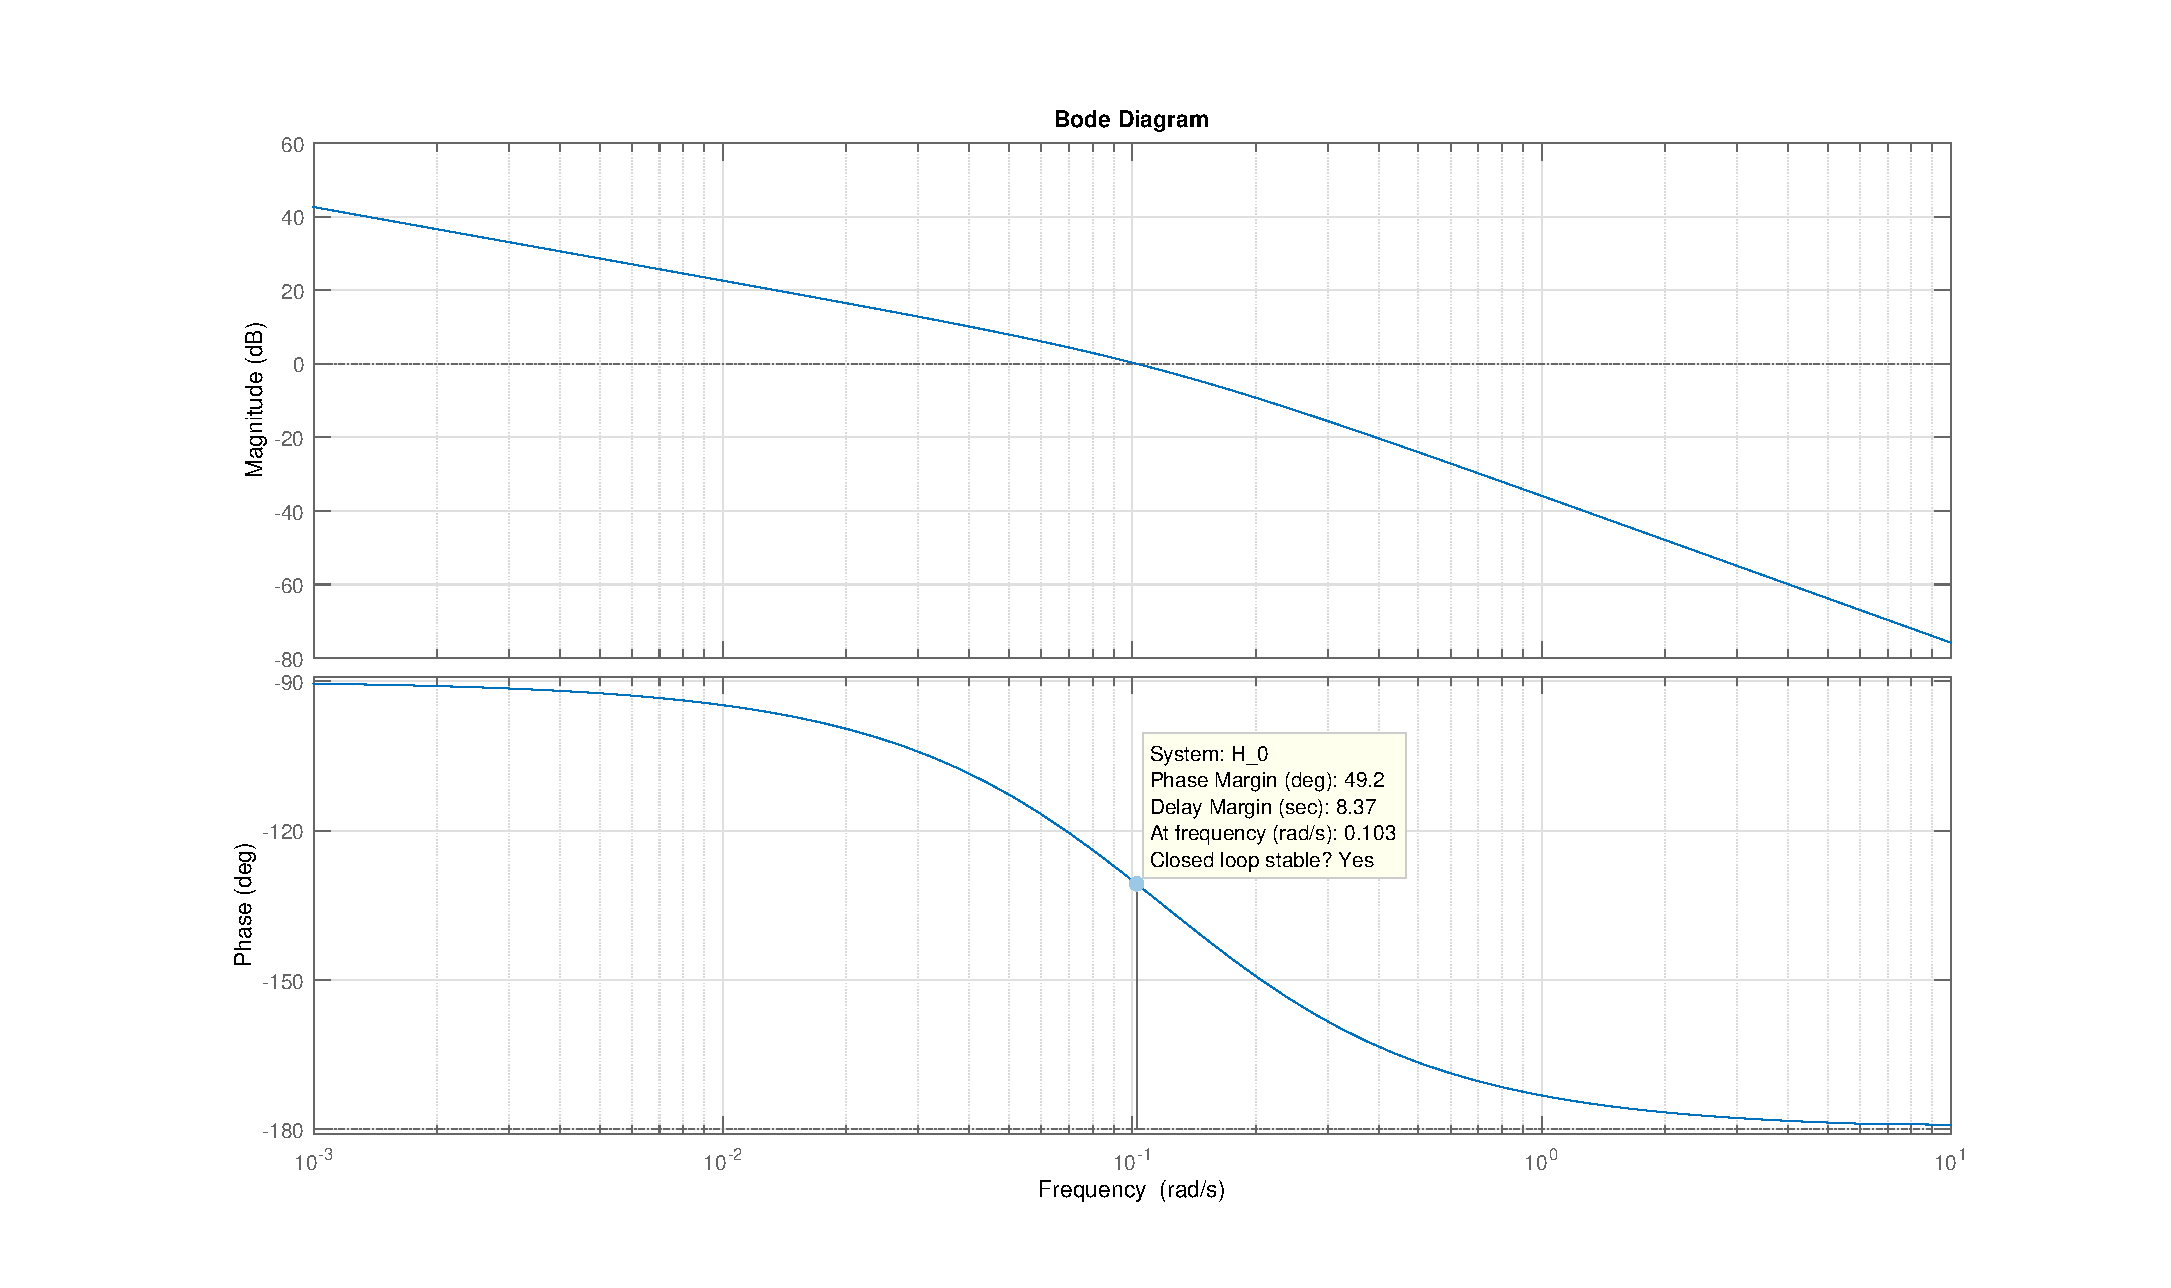
\includegraphics[width=\textwidth]{figures/bode_plot.eps}
	\caption{Bode plot for open loop system transfer function}
\label{fig:p5p3_bode_plot}
\end{figure}


\subsection{Problem b} \label{sec:Autopilot_b}

\begin{figure}[h]
	\centering
	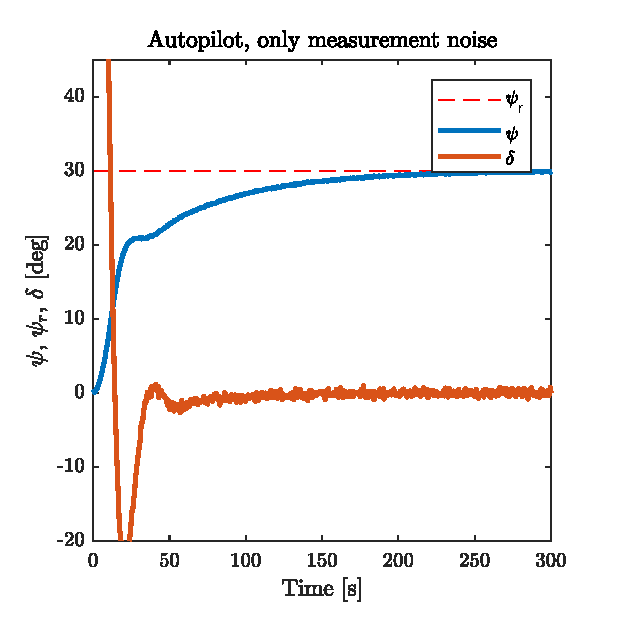
\includegraphics[width=\textwidth]{figures/p5p3b.eps}
	\caption{No disturbances, only measurement noise}
\label{fig:p5p3b_only_noise}
\end{figure}

Simulating the autopilot designed in the previous problem with only measurement noise turned on gives a desired result as seen in \cref{fig:p5p3b_only_noise}. The ship reaches it's set-point for the heading ($\psi_r = 30^\circ$), which is the most important aspect of it. We have not been given any indication of the size of the ship other than it is a \textit{cargo}-ship. At first we thought that 200-250 seconds, about 4 minutes, was a long time to turn a naval vessel, but that might not be the case for the largest of ships.



\subsection{Problem c} \label{sec:Autopilot_c}

\begin{figure}[h]
	\centering
	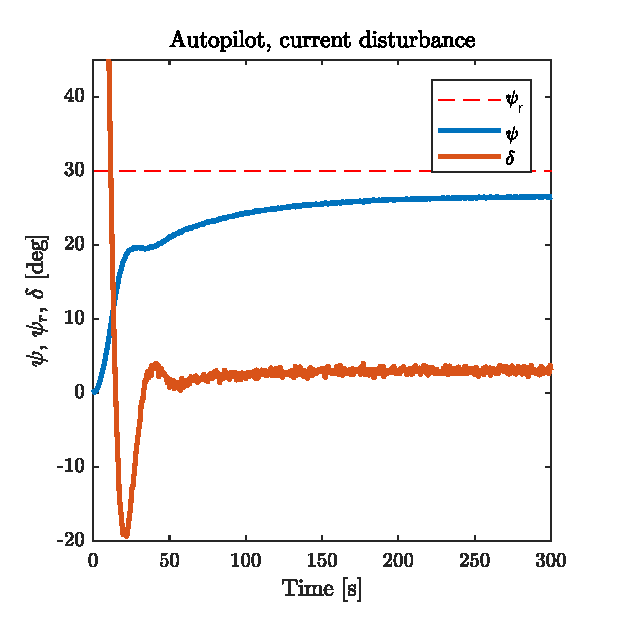
\includegraphics[width=\textwidth]{figures/p5p3c.eps}
	\caption{Current disturbance and measurement noise}
\label{fig:p5p3c_current_distur}
\end{figure}

When we simulate with the current disturbance turned on the ship does not reach it's desired heading as seen in \cref{fig:p5p3c_current_distur}. The stationary error is of about $5^\circ$ which is almost 17 \% of the desired change in heading. Having an error this big with a current disturbance (say the Gulf stream over the Atlantic) would make a ship hit the wrong continent on arrival.


\subsection{Problem d} \label{sec:Autopilot_d}

\begin{figure}[h]
	\centering
	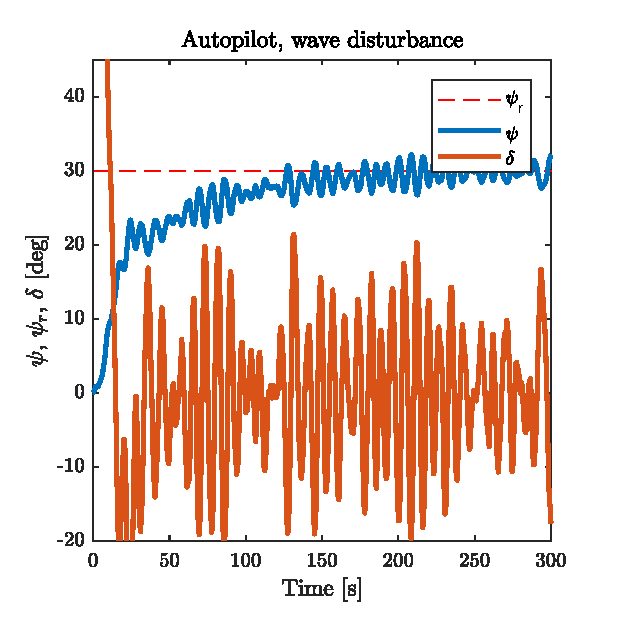
\includegraphics[width=\textwidth]{figures/p5p3d.eps}
	\caption{Wave disturbance and measurement noise}
\label{fig:p5p3d_wave_distur}
\end{figure}

In the simulation of the autopilot with wave disturbance, and no current disturbance, we reach and hold the desired heading, but at a fatal cost. As can be seen in \cref{fig:p5p3d_wave_distur}, the rudder input, $\delta$, is fluctuating very rapidly as the controller is trying to correct the changes in course made by the waves. Making such sudden changes back and forth over a small time-interval when the rudder probably is the size of a bus and has to move an enormous amount of water, will wear out the actuator for the rudder in no time. Changing the actuator every time a voyage is subjected to rough weather is going to be very cost-inefficient and is not an ideal situation.



\subsection{Result evaluation} \label{sec:Autopilot_eval}

Initially, when designing the controller we misinterpreted $\omega_c$ as the \textit{cutoff}-frequency, instead of the \textit{cross}-frequency (which we thought was denoted $\omega_0$ - where the amplitude crosses the 0 dB line in a bode plot, and the amplitude of the transfer function equals 1). This made our design of the controller somewhat different at first, with the values $T_f = 10$ and $K_{pd} = 0.641$. This gave us a phase margin of $\varphi = 51.8^\circ$ at $\omega_{cross} = 0.0786$ rad/s. With these values we had $\omega_{cutoff} = 0.1$ such that $|H(j \omega_{cutoff})| = \frac{1}{\sqrt{2}} = -3$ dB. This was the controller we used in the following assignments until we noticed the possible mistake we had made. We then ran all the simulations again and what we discovered was that our "mistake" actually gave us a seemingly better result than the controller specified in the assignment. In our simulations of problem b in this part of the assignment the response of our initial controller is shown in \cref{fig:p5p3b_OLD}, and the response of the controller specified by the assignment is shown in \cref{fig:p5p3b_only_noise}. Our initial controller reaches the set value marginally faster, has a smoother change in heading and the input, $\delta$ has smaller magnitude with less oscillations. 

Addressing the stationary error caused by a current disturbance can be done by adding an I-term to the PD-controller as it will change input not only in relation to the error but also how long the error has persisted.

The high frequency rudder change while the system is subjected to a wave disturbance can be limited by applying a low-pass filter on the measured heading as the controller will then not register the sudden changes in course, but rather have a more gradual correction, if the waves affect the heading too much.


This leads us to conclude that a better autopilot can be found by spending more resources on the tuning of the PD-controller and determining boat-parameters. Despite our findings we chose to use the controller specified in the assignment text in our final results as Kalman filtering is the main purpose of this assignment, and it will address the issues caused by both sources of disturbance.


Another note on the obtained results is that when our set-point is $\psi_r = 30^\circ$, the controller gives an initial input to the ship at approximately $\delta = 140^\circ$. Due to the saturation in the actual ship-model of $|\delta|_{max} = 45^\circ$, we chose not to saturate the output from the controller so we could see the unsaturated response of our controller.


\begin{figure}[h]
	\centering
	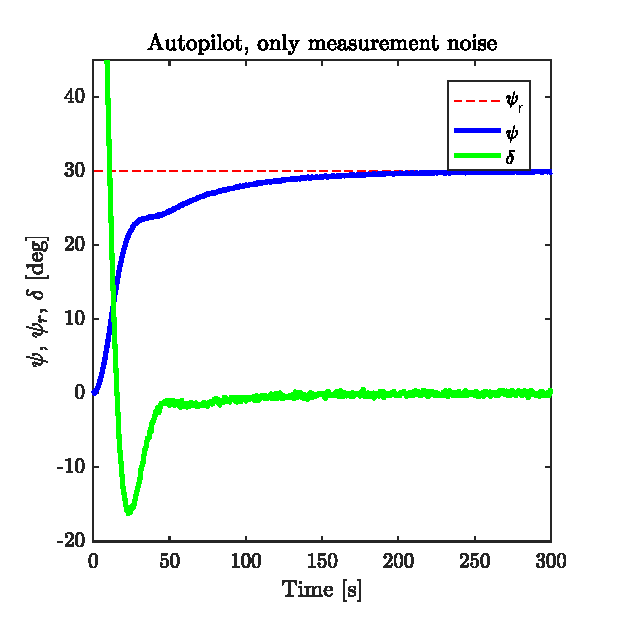
\includegraphics[width=\textwidth]{figures/Ass3_b_only_noise_old.eps}
	\caption{Response of initial controller design without disturbances}
\label{fig:p5p3b_OLD}
\end{figure}